\subsection{Modelling abstractions}\label{subsec:abstractions}

In molecular networks in the cell, cascades of chemical and physical interactions enable propagation of 
signals through the network. In this process, the activity of upstream molecules induces a change in the 
concentration or activity of downstream molecules. For many reactions, the values of the kinetic parameters 
are unknown or difficult to collect. This lack of knowledge hampers the feasibility 
of computational models that describe molecular networks in fine mechanistic detail, especially for larger networks.
As a solution to this problem, we propose the construction of models at a higher level of abstraction, 
thereby reducing the number of parameters involved. In choosing a suitable abstraction level, it is important to 
retain enough descriptive power to give a meaningful formal description of the topology and the 
associated dynamic behavior of biological networks.

As a first abstraction in ANIMO models, the active and inactive forms of each network component 
are represented together by a single node in the network.
Each of these nodes is characterized by its \emph{activity level}, which
represents the fraction of active molecules of that molecular species. When a molecule is known to be 
constitutively active, changes in concentrations of that molecule are treated as changes in its activity level.
Activity levels are discretized into integer variables with a user-defined granularity, ranging from 
Boolean (2 levels) to near-continuous (100 levels).

Detailed biochemical reaction mechanisms are abstracted to \emph{interactions}, which can 
represent either activations ($\rightarrow$) or inhibitions ($\dashv$). 
This aggregation of elementary reactions into single interaction steps reduces the number of kinetic 
parameters involved, while preserving cause-and-effect relationships.
For example, consider a reaction in which enzyme $E$ phosphorylates and activates substrate $S$, 
transferring a phosphate group from a molecule of ATP to a molecule of $S$. Biochemically, this reaction 
can be represented as
$$
\mbox{\it E} + \mbox{\it S} + \mbox{\it ATP} \rightleftarrows \mbox{\it ES} + \mbox{\it ATP} \rightarrow \mbox{\it ES}^{\mbox{\scriptsize \it P}} + \mbox{\it ADP} \rightleftarrows \mbox{\it E} + \mbox{\it S}^{\mbox{\scriptsize\it P}} + \mbox{\it ADP},
$$
with conservation condition $\mbox{\it S}_{\mbox{\scriptsize\it tot}} = \mbox{\it S} + \mbox{\it S}^{\mbox{\scriptsize\it P}}$.\\
In an ANIMO model this reaction is abstracted to the corresponding interaction
$$
\mbox{\it E} \rightarrow \mbox{\it S}.
$$
Each occurrence of the interaction $E \rightarrow S$ will increase the activity level of $S$ by one discrete step. 
Since the activity level is defined as the active fraction of a molecular species, an increase in the active fraction
implies a decrease in the inactive fraction. Hence, the original conservation condition is automatically  
satisfied.
The interaction rate, $R$, depends on the activity levels of the reactants involved and on a single kinetic
parameter $k$ that is set by the user. 
The three available interaction scenarios can be interpreted as abstracted kinetic rate laws:
\begin{enumerate}
  \item $R = k \times [E]$: the interaction rate depends only on the activity level of the upstream node.
  \item $R = k \times [E] \times [1 - S]$ (activations) or $R = k \times [E] \times [S]$ (inhibitions): the rate 
  depends on the activity levels of both the upstream and downstream participants. Activations depend on the 
  presence of inactive substrate, \emph{[1 - S]}, whereas inhibitions depend on the level of active substrate,
  \emph{[S]}.
  \item $R = k \times [E_1] \times [E_2]$: This scenario can be used when the activition or inhibition
  of a downstream node depends on the simultaneous activity of two upstream nodes. This scenario is comparable to an
  \emph{AND-gate} in Boolean logic.
\end{enumerate}
We will show in Section~\ref{sec:results} that the abstraction proposed here preserves ample
expressivity to capture the dynamic behavior of a biological network. 


\subsection{Modelling interactions with Timed Automata}\label{subsec:timed-automata}
\def\ta{TA}
\def\tas{TA}

Timed Automata have been shown to be a powerful formalism to model biological processes
~\citep{ta-siebert,bartocci-oscillators,oded-ode-ta-discretization}. A timed automaton consists of locations
and transitions between these locations~\ref{fig:abstraction-mek-erk} and a system of timed automata can be 
used to model a system of interacting molecules. At any time, each automaton is in a specific location, and together 
these locations corresponds to a state of the biological system. Each timed automaton has a local clock 
associated to it, allowing temporal control of transitions between locations. These transitions are used to 
represent interactions between molecules. Fast interactions take less time than slow interactions 
to perform each activation or inhibition step. We have previously described in detail how the 
scenarios presented in Sect.~\ref{subsec:abstractions} can be used to calculate the timing of molecular 
interactions to give a description of network dynamics (@@Ref Bibe@@). An example of a small Timed Automata model 
illustrates the basic properties of \tas\~\ref{fig:abstraction-mek-erk}. 
This model describes the activation of extracellular regulated kinase (ERK) by MAPK ERK kinase (MEK).


\def\mekTA{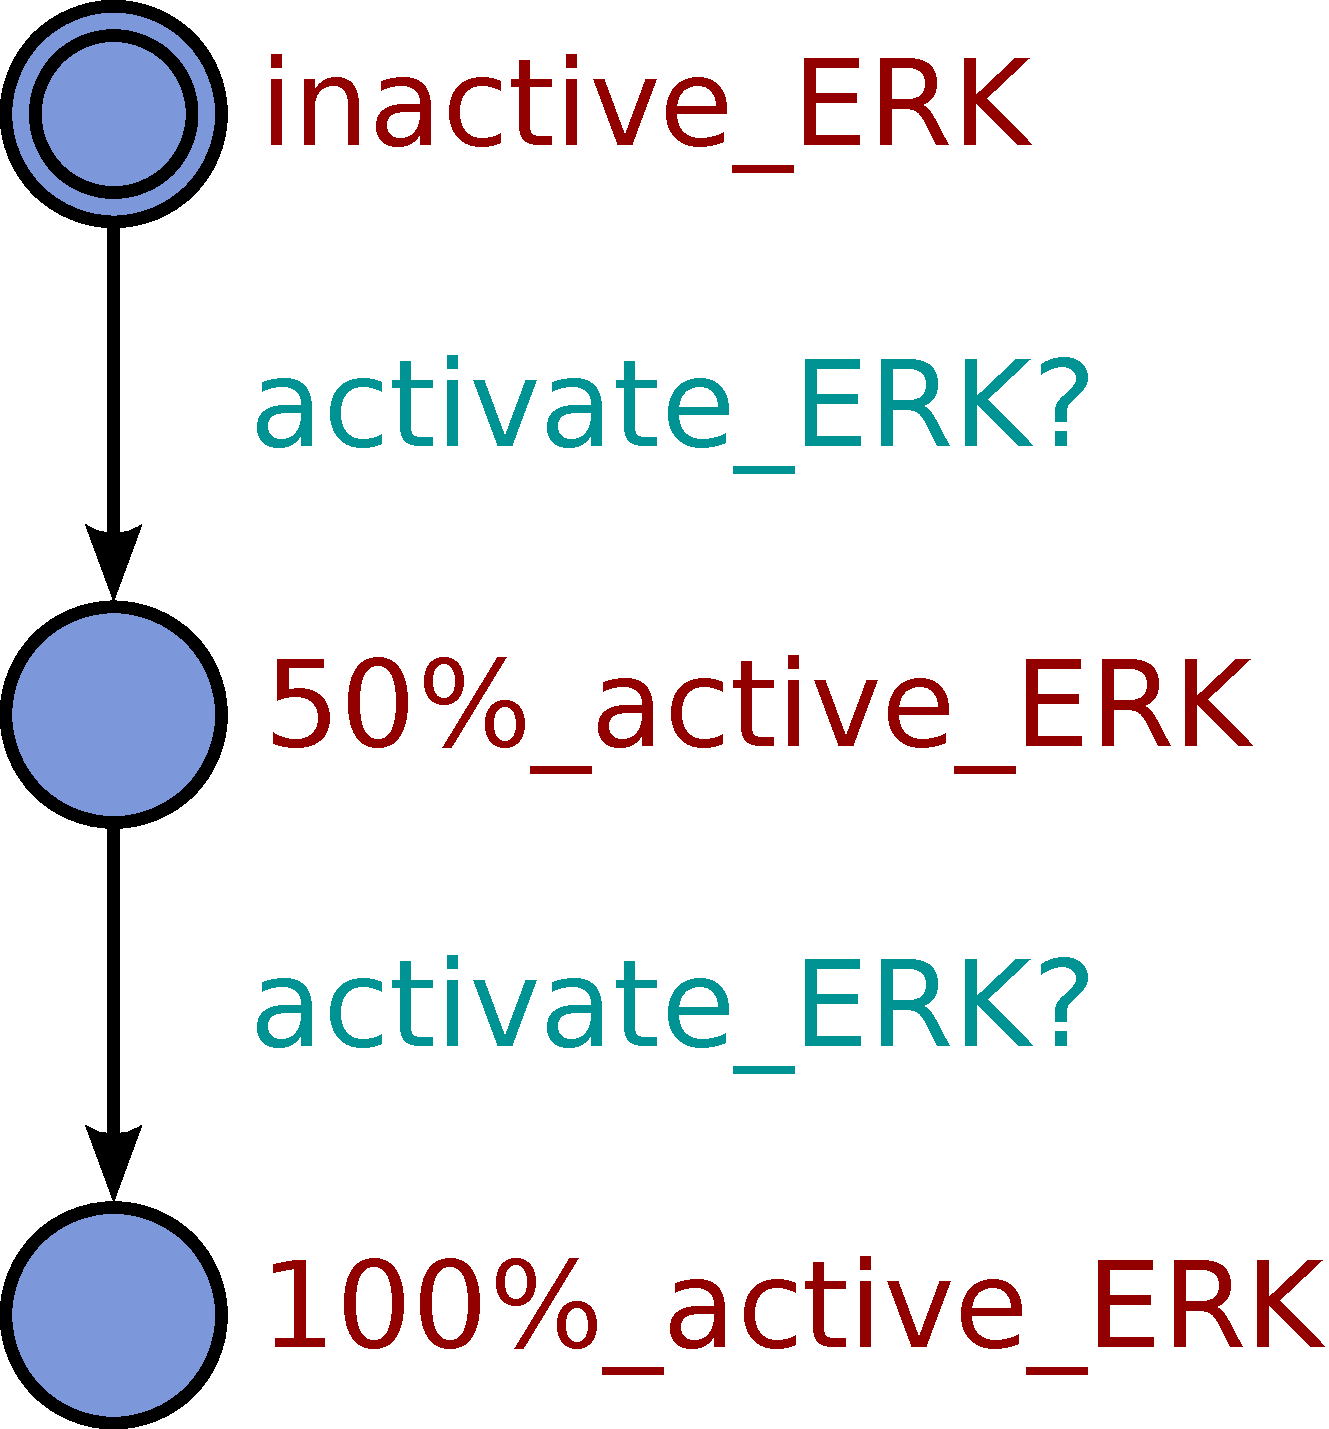
\includegraphics[scale=.098]{images/abstraction_ta_erk3}}
\newlength\mekTAheight
\setlength\mekTAheight{\heightof{\mekTA}}
\begin{figure}[!hb]
%\begin{minipage}{\textwidth}
\begin{center}
\subfloat[\label{subfig:mek-erk}]{\begin{minipage}[c][\mekTAheight]{0.13\textwidth}\begin{center}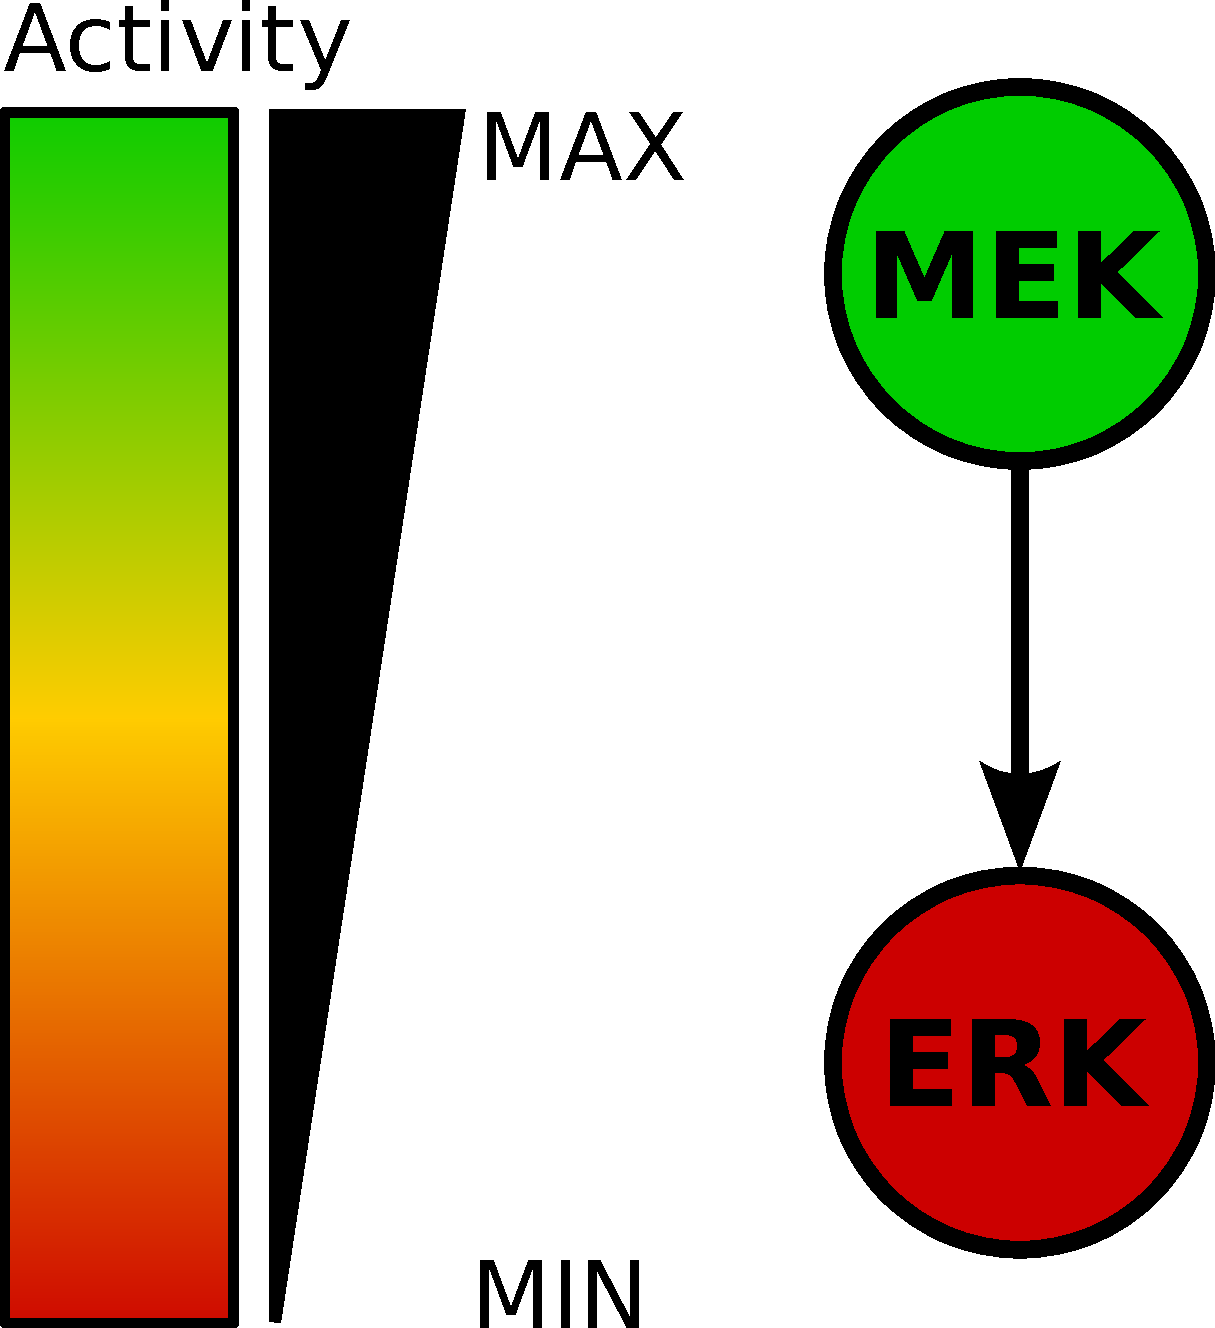
\includegraphics[scale=.098]{images/abstraction_ta_mek-erk3}\end{center}\end{minipage}}
\qquad
\subfloat[\label{subfig:mek}]{\begin{minipage}[c][\mekTAheight]{0.13\textwidth}\begin{center}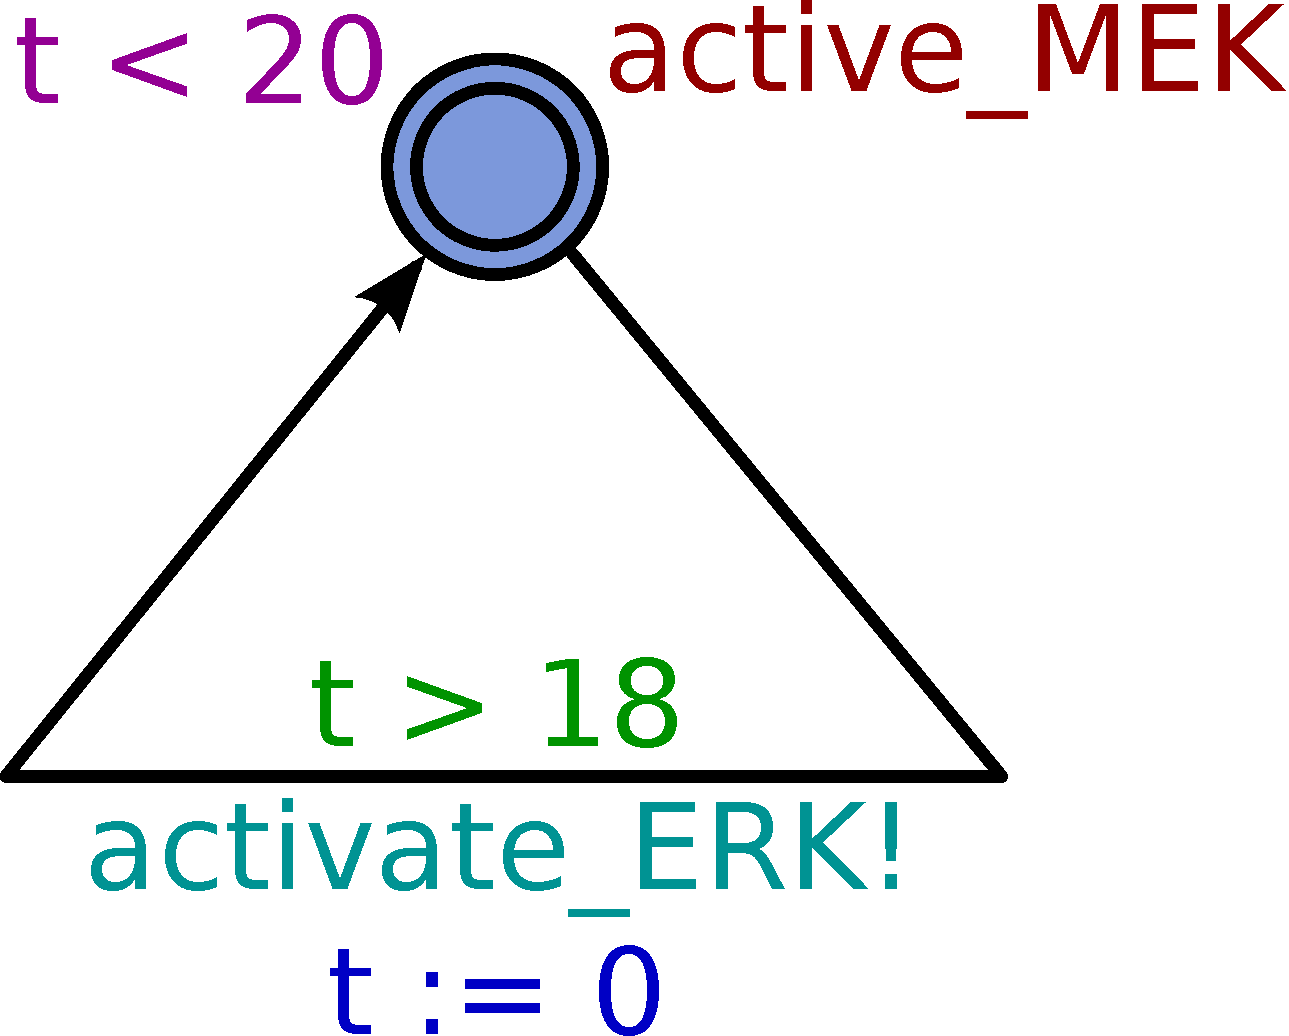
\includegraphics[scale=.098]{images/abstraction_ta_mek}\end{center}\end{minipage}}
\qquad
\subfloat[\label{subfig:erk}]{\begin{minipage}[c][\mekTAheight]{0.14\textwidth}\begin{center}\mekTA\end{center}\end{minipage}}
\end{center}
\caption{Parallel between an abstract activation interaction and its \tas\ model.
{\bf \protect\subref{subfig:mek-erk}}~Classical depiction of a well-studied intracellular signal transduction interaction: protein
MAPK-ERK kinase (MEK, active) activates downstream protein extracellular-regulated kinase (ERK, initially inactive).
In this example, MEK activity is not regulated and ERK has three activity levels,
completely inactive, halfway active and completely active.
{\bf \protect\subref{subfig:mek}}~A \ta\ model of active MEK, consisting of one location (circle) and one
transition (arrow). ${\sf t} < 20$ is termed an invariant on the location, allowing residence in this location as long as local
clock time {\sf t} is smaller than $20$ units. ${\sf t} > 18$ is termed a guard on the transition, allowing the
transition to take place when local clock {\sf t} is greater than $18$ units. Together, the invariant and guard in this
example ensure that the transition must take place within the (continuous) time interval $18 < {\sf t} < 20$. When the
transition takes place, the action {\sf activate\_Erk!} is performed (thus allowing the ERK automaton to reach the {\sf
50\%\_active\_ERK} location) and the local clock coupled to this automaton is reset, ${\sf t} := 0$.
This allows the reaction to occur another time, fully activating ERK.
{\bf \protect\subref{subfig:erk}}~A \ta\ model of ERK, consisting of three locations, {\sf inactive\_ERK}
(the starting location), {\sf 50\%\_active\_ERK} and {\sf 100\%\_active\_ERK},
and two transitions between the locations. A transition will take place when it is possible to synchronize with
the corresponding action {\sf activate\_ERK!} in the MEK automaton.
Each synchronization on channel {\sf activate\_ERK} represents the occurrence of the activating
interaction between MEK and ERK, and allows ERK to eventually become completely active.}\label{fig:abstraction-mek-erk}
%\end{minipage}
\end{figure}





\subsection{ANIMO}
The modelling approach described in Section~\ref{subsec:abstractions} is implemented in the
software tool ANIMO (Analysis of Networks with Interactive MOdelling, \citealt{animo-bibe}),
a plug-in to the network visualization tool Cytoscape~\citep{cytoscape}. The visual interface of ANIMO
is designed to allow the user to intuitively construct activity-based models, making the expansion
and rewiring of a network a fast and user-friendly process (see Suppl. Video 1). An ANIMO model can
be analysed through simulation, with the results automatically plotted as a graph.
The dynamic behaviour of a model can then be interactively explored by
acting on a slider to highlight time points in a simulation. The selected simulation
point defines the appearance of the network: each node will be coloured depending on its activity level
at the selected simulation instant. Moreover, experimental data can be matched against
the predictions of a model, superposing time-based activity series to a graph produced from the model.


Each network built with ANIMO is automatically translated to
a \tas\ model, which is then simulated with the model checking tool UPPAAL~\citep{uppaal},
translating back the results in the proper user-friendly format
(all parts of Figure~\ref{fig:small-model}, as well as similar figures
in the rest of the paper, were taken from ANIMO's user interface).
No training
or prior knowledge on the use of \tas\ or UPPAAL is needed in order to benefit from ANIMO.
Nevertheless, the translation process can be followed in a transparent manner if
desired by the user.

The technical foundations of ANIMO have been described by us elsewhere~\citep{animo-bibe}. 
An abstract overview on the \tas\ model can be found in Supplementary Section~\ref{suppl-sec:animo-ta}.


\subsection{Using ANIMO to build a model based on data}\label{subsec:case-study}
To illustrate the process of model building in ANIMO, we consider now an example based on a literature compendium of
signal transduction events in HT-29 human colon carcinoma cells~\citep{pathway-compendium}. This data set comprises triplicate
measurements of 11 different protein activities or post-translational modification states at 13 time points after
treatment with different combinations of tumour necrosis factor-$\alpha$ (TNF$\alpha$), epidermal growth factor (EGF) and insulin.
The data set contains relative protein levels and activities, and no absolute quantities, which is the typical situation in biochemistry.

As a first step, we normalized measurements for each protein to the
maximum value in the complete experiment, resulting in a nondimensionalized data set that is suitable for use with ANIMO.


In Figure~\ref{fig:small-model}, we show the stepwise construction of a model of a small part of the network that is
able to account for measured variations in activity of inhibitor of nuclear factor kappa-B kinase (IKK), c-Jun N-terminal kinase-1 (JNK1),
mitogen-activated protein kinase-activated protein kinase 2 (MK2), Caspase 8 (Casp8) and Caspase 3 (Casp3) upon stimulation with 100
ng/ml TNF$\alpha$. In this example we aimed for inclusion of a minimum number of nodes in the network, while preserving biological relationships.
Multi-step cascades were aggregated into a single step when possible. Parameters for all reactions were set manually, resulting in a close
match between the model and the patterns observed in the dataset.

A more comprehensive version of this model is presented in Section~\ref{subsec:case-study-larger}.

\def\modelGraphScale{0.2}%0.148}%0.215}
\def\legendGraphScale{0.23}%0.16}
\def\halfGraphScale{0.09}%0.067}%0.1075}
\begin{figure}[!bhtp]
\centering
\begin{tabular}{ll}
\subfloat{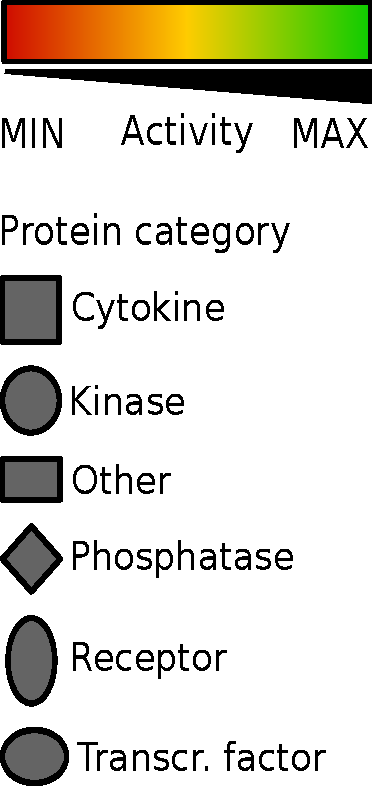
\includegraphics[scale=\legendGraphScale]{images/small-model-1g_legenda}}\addtocounter{subfigure}{-1}\subfloat[\label{fig:small-model-first}]{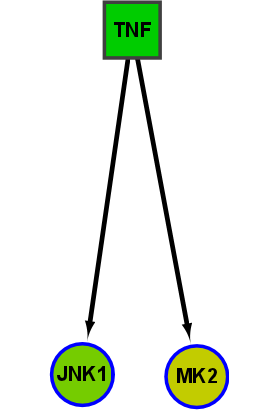
\includegraphics[scale=\modelGraphScale]{images/00-paper-model1f}}
& \subfloat[\label{fig:small-model-first-graph}]{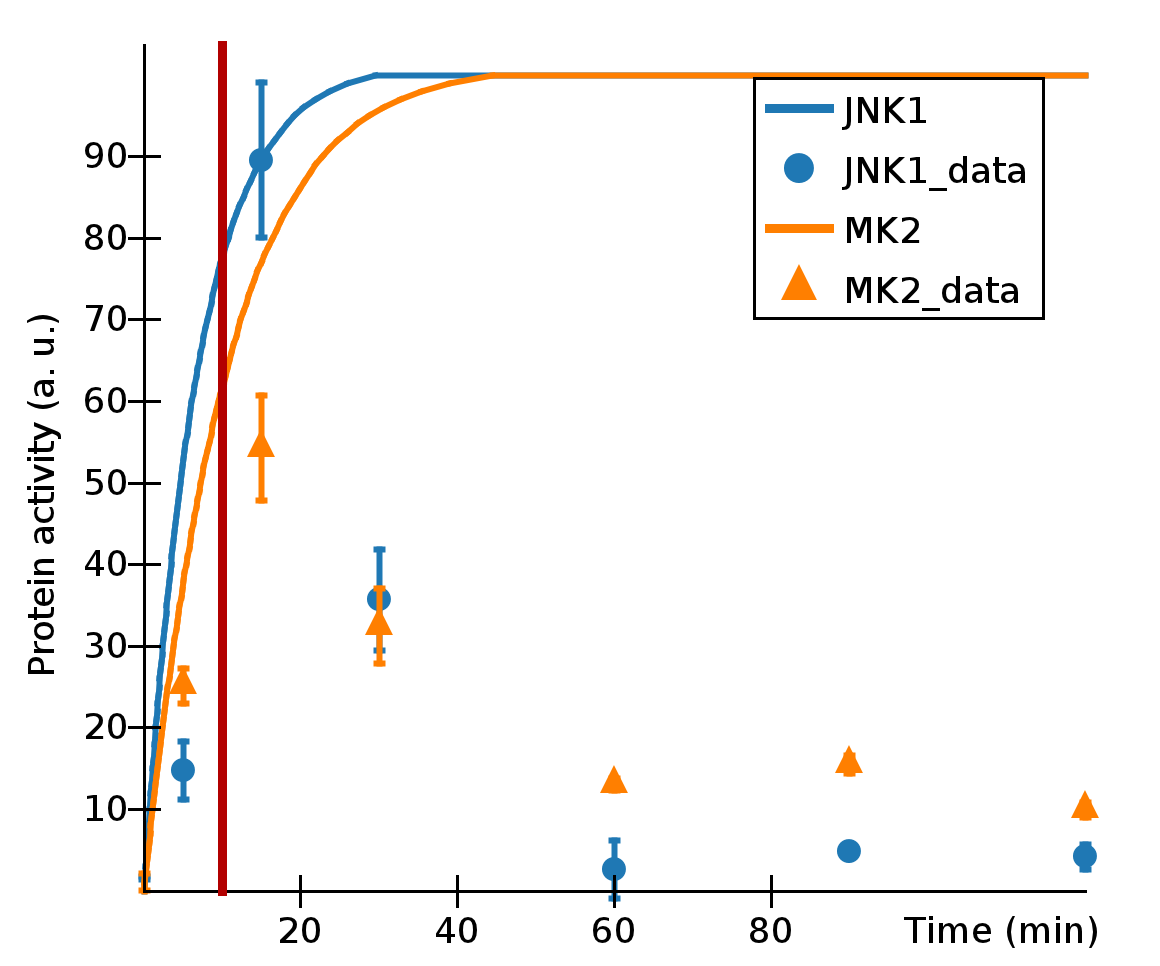
\includegraphics[scale=\halfGraphScale]{images/00-paper-graph1m_riga}} \\[5ex]
\subfloat[\label{fig:small-model-third}]{\qquad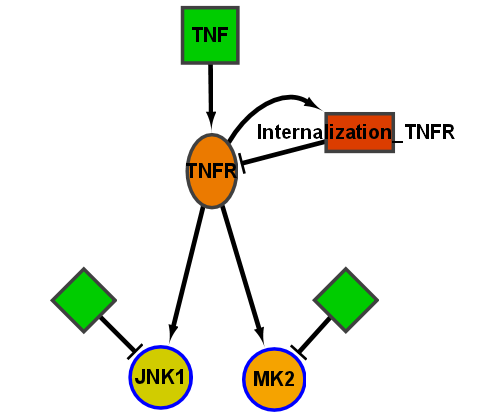
\includegraphics[scale=\modelGraphScale]{images/00-paper-model3f}}
& \subfloat[\label{fig:small-model-third-graph}]{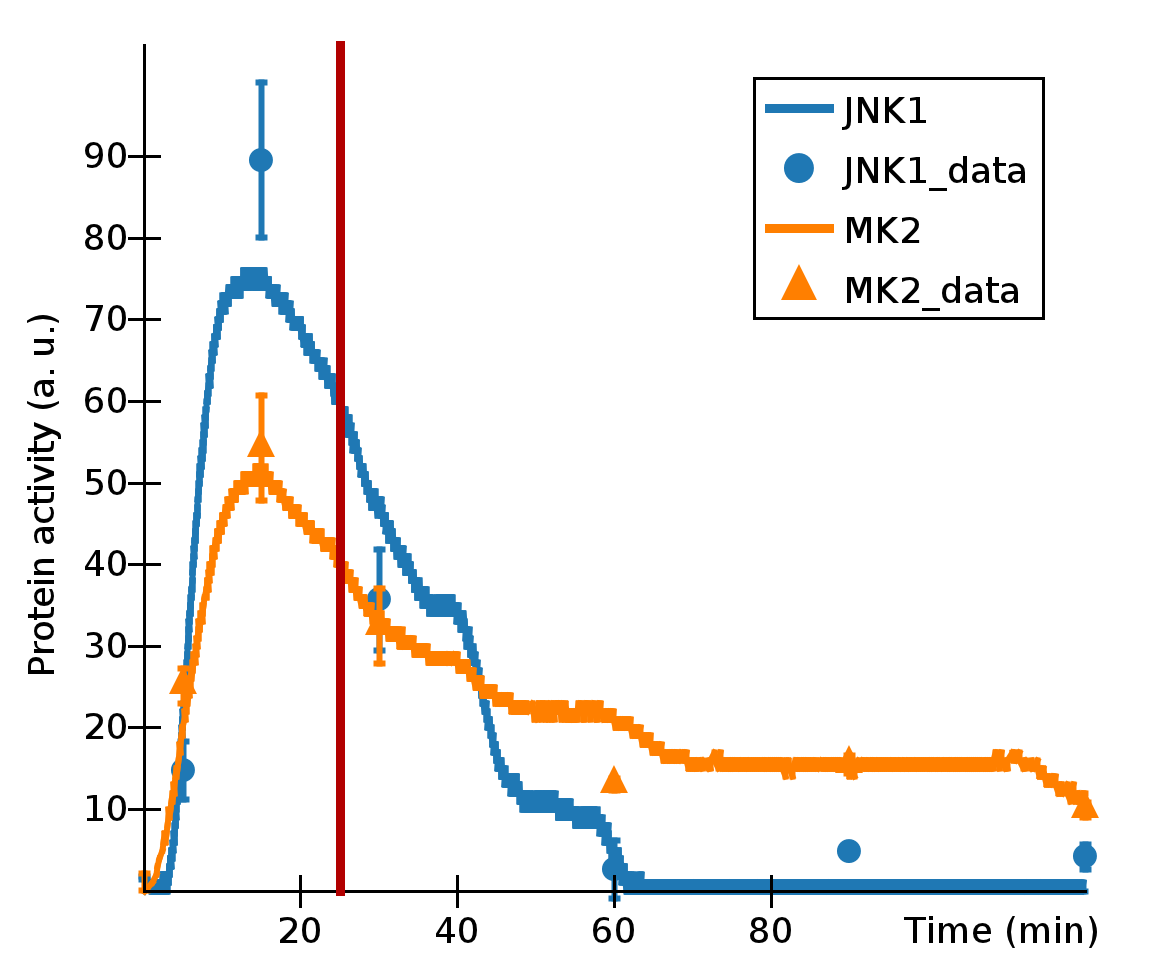
\includegraphics[scale=\halfGraphScale]{images/00-paper-graph3n_riga}} \\[5ex]
\subfloat[\label{fig:small-model-fourth}]{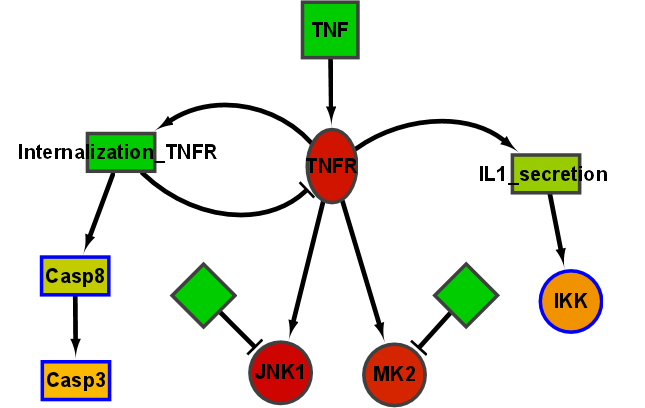
\includegraphics[scale=\modelGraphScale]{images/00-paper-model4g}}
& \subfloat[\label{fig:small-model-fourth-graph}]{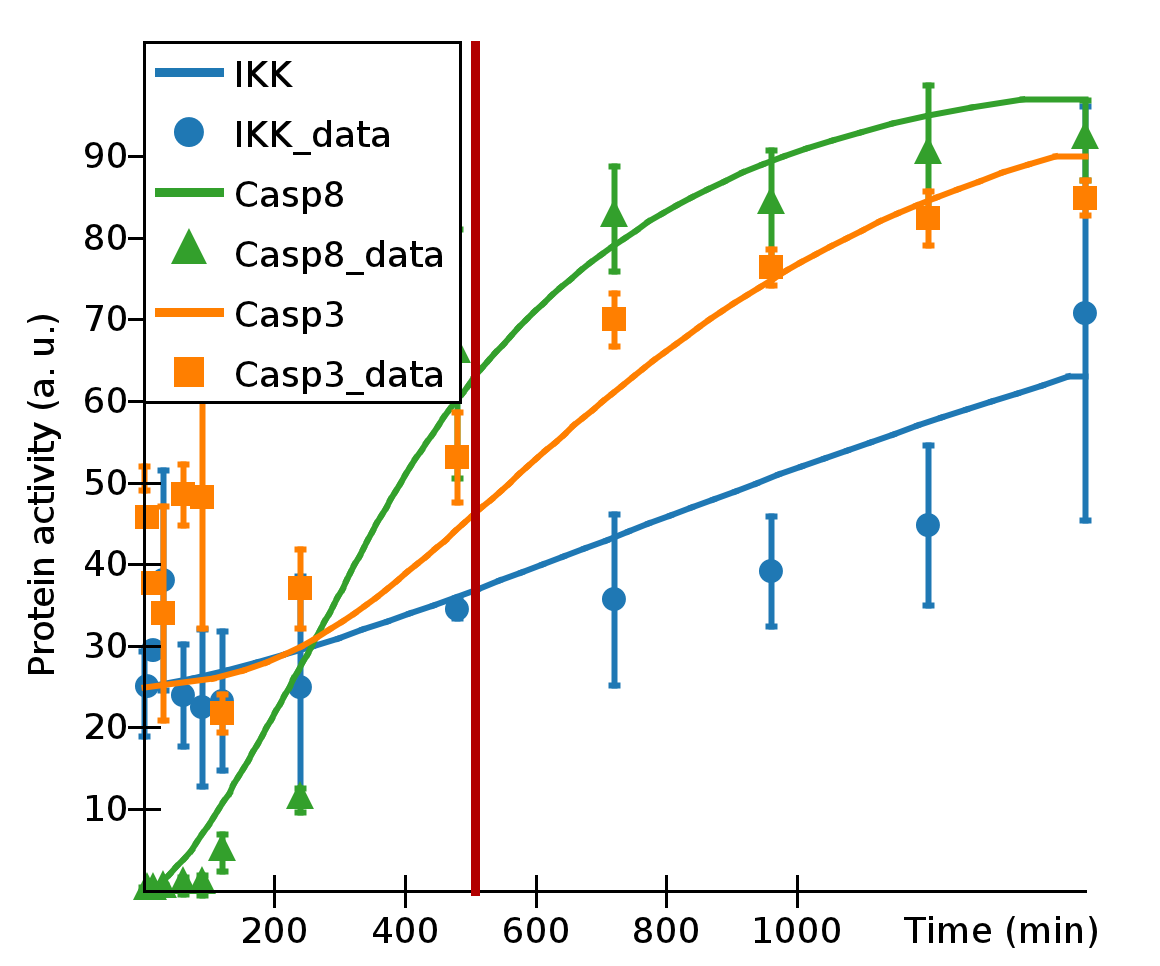
\includegraphics[scale=\halfGraphScale]{images/00-paper-graph4o_riga}}
\end{tabular}
  \caption{
Incremental construction of an ANIMO model of signal transduction
events in human colon carcinoma cells upon stimulation with 100 ng/ml TNF$\alpha$.
Each construction step (top to bottom) is simulated in ANIMO, giving intermediate feedback
useful for the piecewise refinement of the model.
The graphs on the right show the dynamic behaviour of the corresponding models on the left, comparing it to the measured
activity values by~\cite{pathway-compendium} (error bars represent the standard deviation).
On the vertical axis, ``100'' represents the maximum protein activity in the complete experiment.
A red vertical line in each graph highlights a selected time point in the time course:
nodes in the corresponding model are coloured according to their activity at that time point.
{\bf (\protect\subref*{fig:small-model-first}, \protect\subref*{fig:small-model-first-graph})}~Basic model showing direct activation of JNK1 and MK2 by TNF$\alpha$.
No peak dynamics are observed because no inactivating processes are present.
{\bf (\protect\subref*{fig:small-model-third}, \protect\subref*{fig:small-model-third-graph})}~The model after addition of inactivating phosphatases and a
negative feedback loop that down-regulates TNFR (TNF receptor). Note that adding TNFR internalization or phosphatases alone would not be enough to reproduce activity peaks.
{\bf (\protect\subref*{fig:small-model-fourth}, \protect\subref*{fig:small-model-fourth-graph})}~The model after addition of IKK, IL1-secretion (abstracting
the autocrine IL-1 signalling described by~\citealp{pathway-autocrine}), Casp8 and Casp3, showing the late response to TNF$\alpha$ signalling.
As the data set did not contain values for cleaved caspase-3, but only for its non-cleaved precursor pro-caspase-3,
we computed the {\sf Casp3\_{}data} series as $100\% - [\mbox{\sf pro-Casp3}]$.}\label{fig:small-model}
\end{figure}
